\documentclass[11pt,a4paper]{article}
\usepackage[margin=2.2cm]{geometry}
\usepackage[T1]{fontenc}
\usepackage[utf8]{inputenc}
\usepackage{lmodern}
\usepackage{microtype}
\usepackage{graphicx}
\usepackage{booktabs}
\usepackage{longtable}
\usepackage{array}
\usepackage{tabularx}
\usepackage{xcolor}
\usepackage{listings}
\usepackage{amsmath,amssymb}
\usepackage{enumitem}
\usepackage{fancyhdr}
\usepackage{hyperref}
\usepackage{caption}
\usepackage{float}
\usepackage{parskip}
\usepackage{lastpage}

\definecolor{mmalsblue}{HTML}{17365D}
\definecolor{mmalsgreen}{HTML}{2F6B4F}
\definecolor{mmalsorange}{HTML}{9A4F13}
\definecolor{lightgray}{HTML}{F3F5F7}
\definecolor{codegray}{HTML}{F7F7F7}

\hypersetup{
  colorlinks=true,
  linkcolor=mmalsblue,
  urlcolor=mmalsblue,
  citecolor=mmalsblue,
  pdftitle={MMALS RC2O-v2.3.2 Per-Sample Context Fusion Repair - Change Report},
  pdfauthor={MMALS Project}
}

\pagestyle{fancy}
\fancyhf{}
\lhead{MMALS RC2O-v2.3.2}
\rhead{Reviewer Change Report}
\cfoot{\thepage\ of \pageref{LastPage}}
\setlength{\headheight}{14pt}

\lstdefinestyle{pythonstyle}{
  language=Python,
  backgroundcolor=\color{codegray},
  basicstyle=\ttfamily\footnotesize,
  keywordstyle=\color{mmalsblue}\bfseries,
  commentstyle=\color{mmalsgreen},
  stringstyle=\color{mmalsorange},
  numbers=left,
  numberstyle=\tiny\color{gray},
  numbersep=8pt,
  frame=single,
  rulecolor=\color{gray!35},
  breaklines=true,
  showstringspaces=false,
  tabsize=4,
  columns=fullflexible
}
\lstset{style=pythonstyle}

\newcommand{\code}[1]{\texttt{#1}}
\newcommand{\statusbox}[2]{%
  \begin{center}
  \fcolorbox{#1}{#1!7}{\parbox{0.92\textwidth}{\textbf{#2}}}
  \end{center}
}

\title{\vspace{-1.2cm}\textbf{MMALS RC2O-v2.3.2}\\
\Large Per-Sample Stable-Plastic Context Fusion Repair\\
\large Design, History, Tracked Changes, and Reviewer Archive Report}
\author{MMALS Project Research Artifact}
\date{13 June 2026}

\begin{document}
\maketitle

\statusbox{mmalsorange}{Status: unexecuted diagnostic ablation design. This document archives the completed RC2O-v2.3.1 evidence and the code-level rationale for RC2O-v2.3.2. It does not report a v2.3.2 experimental result.}

\begin{abstract}
RC2O-v2.3.1 introduced a dataset-agnostic stable-plastic context-memory layer for MMALS and produced a meaningful but non-promotable CORe50 result. Across seeds 0 and 4, its principal candidate improved oldest-context recognition, weakest-task retention, class coverage, forgetting, and host diversity. However, the adaptive fusion gate assigned approximately 98.4\% of its mass to the per-sample single-input context branch, while stronger prototype evidence already existed inside the model. The deployed context posterior reached 0.4788 top-1 accuracy, compared with 0.7692 for the best component branch, and recent-task accuracy regressed beyond the predefined tolerance.

This report documents RC2O-v2.3.2, a localized fusion repair. The new notebook preserves exact legacy batch-Fr\'echet inference, adds per-sample diagonal-Gaussian prototype evidence, introduces a stationary stable bank in the representation entering MMALS, adds fixed-fusion controls, constrains adaptive fusion with a prior and residual floor, routes the main non-legacy task loss through the deployed posterior, and adds reviewer gates for branch underperformance and fusion collapse. The artifact is designed to be archived with the notebook and compact predecessor evidence in a GitHub repository.
\end{abstract}

\tableofcontents
\newpage

\section{Artifact identity and scope}

\begin{tabularx}{\textwidth}{>{\bfseries}p{4.1cm}X}
Notebook & {\small\nolinkurl{MMALS_Prototype_1_1_RC2O_v2_3_2_Per_Sample_Stable_Plastic_Context_Fusion_Repair_Ablation.ipynb}} \\
Predecessor & RC2O-v2.3.1 stable-plastic context-memory ablation \\
Primary dataset for mechanism test & CORe50 \\
Initial seeds & 0 and 4 \\
Status & Unexecuted diagnostic design \\
Primary claim boundary & No robust qualification, no universal continual-learning claim, no positive backward-transfer claim \\
Compatibility requirement & Exact historical legacy mode remains callable without reopening old notebooks \\
\end{tabularx}

The change is intentionally local. It does not replace the MMALS hosts, fungal transformations, router, global readout, replay budget, or frozen external visual representation. It modifies the context-memory evidence interface and how that evidence is fused.

\section{Research history}

\begin{longtable}{p{2.8cm}p{5.2cm}p{6.2cm}}
\toprule
\textbf{Version} & \textbf{Question} & \textbf{Outcome carried forward} \\
\midrule
\endfirsthead
\toprule
\textbf{Version} & \textbf{Question} & \textbf{Outcome carried forward} \\
\midrule
\endhead
RC2O-v2.2c & Can selected-policy specialization transfer beyond the MNIST family? & SplitCIFAR10 became the strongest qualified external bridge. SplitCIFAR100 and CORe50 remained diagnostic. \\
RC2O-v2.3 & Can replay, readout and context-retention rescue CORe50? & Average retention and host use improved, but the oldest contexts remained unrecovered. \\
RC2O-v2.3.1 & Can stable-plastic context memory recover old contexts? & Old-context retention improved, but adaptive fusion collapsed toward \code{q\_single}; recent-task performance regressed. \\
RC2O-v2.3.2 & Can per-sample prototype evidence and stationary stable coordinates repair fusion? & Defined by the new notebook. No result is claimed before execution. \\
\bottomrule
\end{longtable}

\section{Completed RC2O-v2.3.1 evidence}

\subsection{Two-seed summary}

\begin{table}[H]
\centering
\small
\begin{tabular}{lrrrrrr}
\toprule
\textbf{Variant} & \textbf{Avg acc.} & \textbf{Oldest 2} & \textbf{Old ctx.} & \textbf{Recent 2} & \textbf{Zero recall} & \textbf{Forgetting} \\
\midrule
Legacy reference & 0.2844 & 0.0469 & 0.0000 & 0.3948 & 4.0 & 0.2012 \\
Current context EMA & 0.2646 & 0.0286 & 0.0000 & 0.3679 & 5.0 & 0.1995 \\
Deployed-posterior distill & 0.2961 & 0.0476 & 0.0320 & 0.3841 & 3.0 & 0.1805 \\
Stable-plastic + distill & 0.2876 & 0.0936 & 0.2104 & 0.3425 & 1.0 & 0.1379 \\
Oracle diagnostic & 0.3223 & 0.1368 & 1.0000 & 0.3994 & 0.5 & 0.1524 \\
\bottomrule
\end{tabular}
\caption{RC2O-v2.3.1 CORe50 means over seeds 0 and 4. The oracle row is diagnostic only.}
\end{table}

The stable-plastic candidate produced a real retention effect: oldest-two context top-1 improved by 0.2104, oldest-two task accuracy improved by 0.0468, zero-recall classes fell by three, and average forgetting fell by approximately 0.0634. It nevertheless failed promotion because recent-two accuracy regressed by 0.0523 and confident-collapse reduction was negligible.

\begin{figure}[H]
\centering
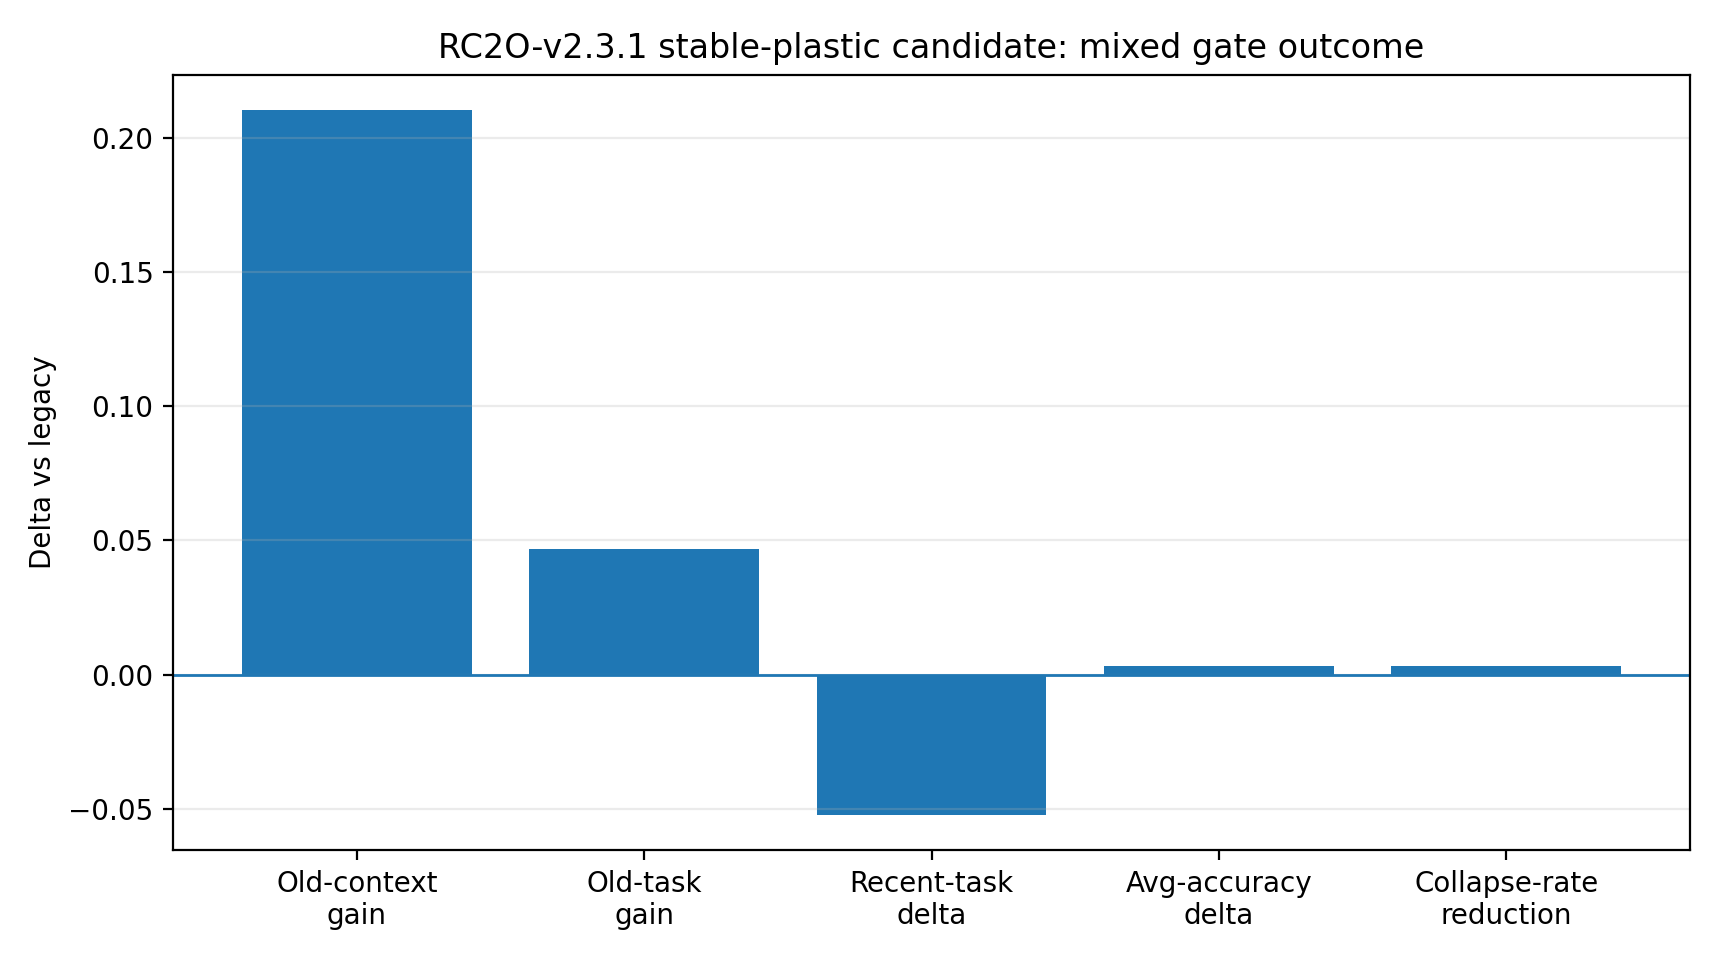
\includegraphics[width=0.90\textwidth]{../figures/v231_gate_outcome.png}
\caption{The v2.3.1 candidate improved old-context and old-task retention but violated recent-task and collapse-reduction criteria.}
\end{figure}

\subsection{Internal evidence exceeded deployed fusion}

\begin{table}[H]
\centering
\small
\begin{tabular}{lr}
\toprule
\textbf{Branch, stable-plastic candidate} & \textbf{Context top-1} \\
\midrule
Single-input context encoder & 0.4195 \\
Feature prototype & 0.7692 \\
Latent prototype & 0.7000 \\
Plastic prototype & 0.6968 \\
Stable prototype & 0.6596 \\
Deployed fused posterior & 0.4788 \\
\bottomrule
\end{tabular}
\caption{The fused posterior was substantially worse than evidence already available inside the model.}
\end{table}

\begin{figure}[H]
\centering
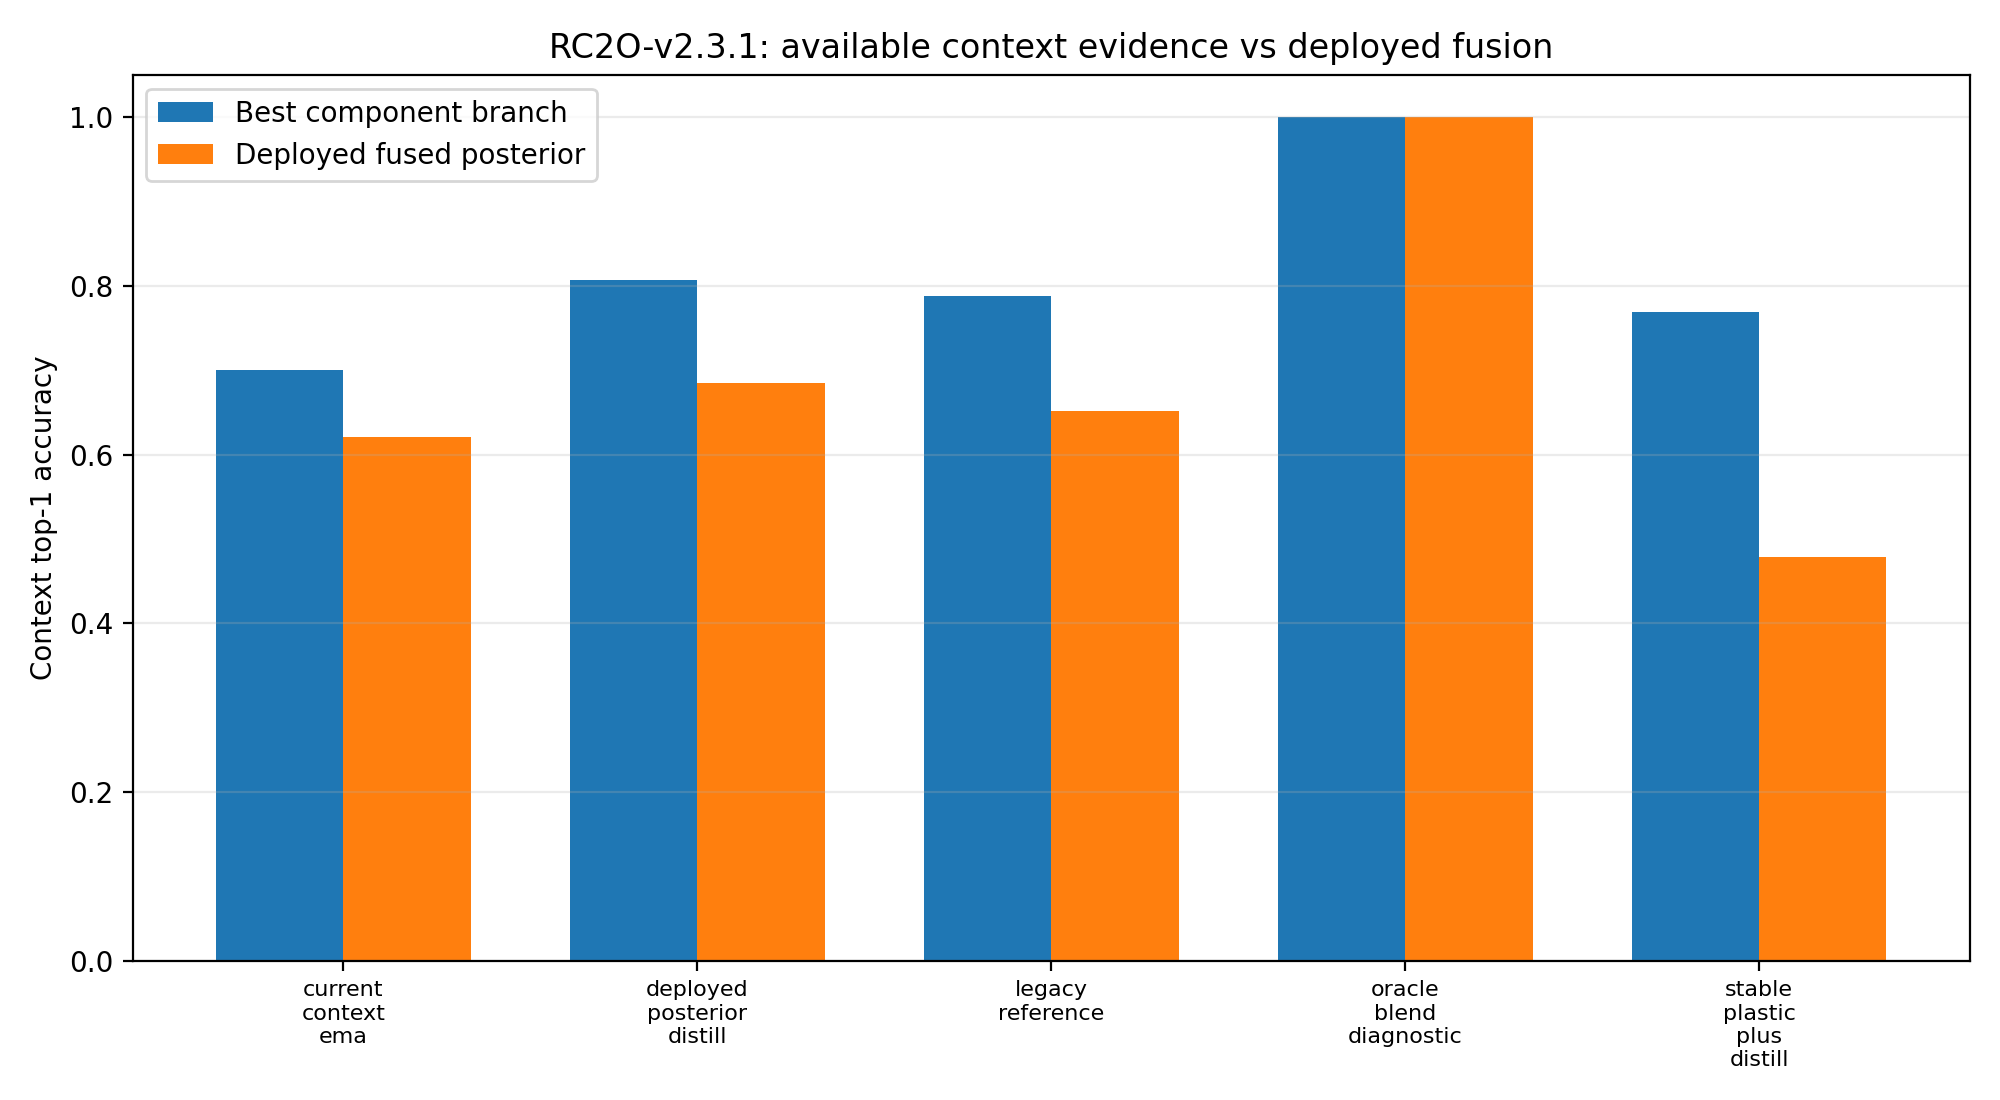
\includegraphics[width=0.96\textwidth]{../figures/v231_best_branch_vs_deployed.png}
\caption{Across v2.3.1 variants, internal component evidence versus the deployed fused posterior. The largest mismatch occurs in the stable-plastic candidate.}
\end{figure}

The average fusion weights of the stable-plastic candidate were approximately 98.4\% single-input, 1.1\% plastic, and 0.5\% stable. This is not interpreted as proof that prototypes are useless. The component accuracies show the opposite. It is interpreted as a training-interface failure.

\section{Root-cause analysis}

\subsection{Batch-level posterior copied across mixed replay}

In v2.3.1, the prototype branch first computed a single Fr\'echet distance per context from the statistics of the entire batch. It then converted those context distances into one posterior vector and expanded that vector over all examples. A task-balanced replay batch can contain samples from several contexts. Therefore, one copied prototype posterior cannot be correct for each item simultaneously.

The single-input branch, by contrast, already produced one posterior per item. During deployed-posterior cross-entropy training, the simplest optimization path was to suppress the incompatible batch-level branches and rely on \code{q\_single}.

\subsection{Stable values in a drifting coordinate system}

The v2.3.1 stable bank stored statistics in learned context-feature and mediated-latent coordinates. Those coordinates continue to move during sequential training. Freezing or slowly updating a prototype does not make its meaning stable when the function that produces the coordinate changes. This is consistent with the broader MMALS lesson that preserving a route or coordinate is not equivalent to preserving the function computed through it.

\section{RC2O-v2.3.2 architecture}

\begin{figure}[H]
\centering
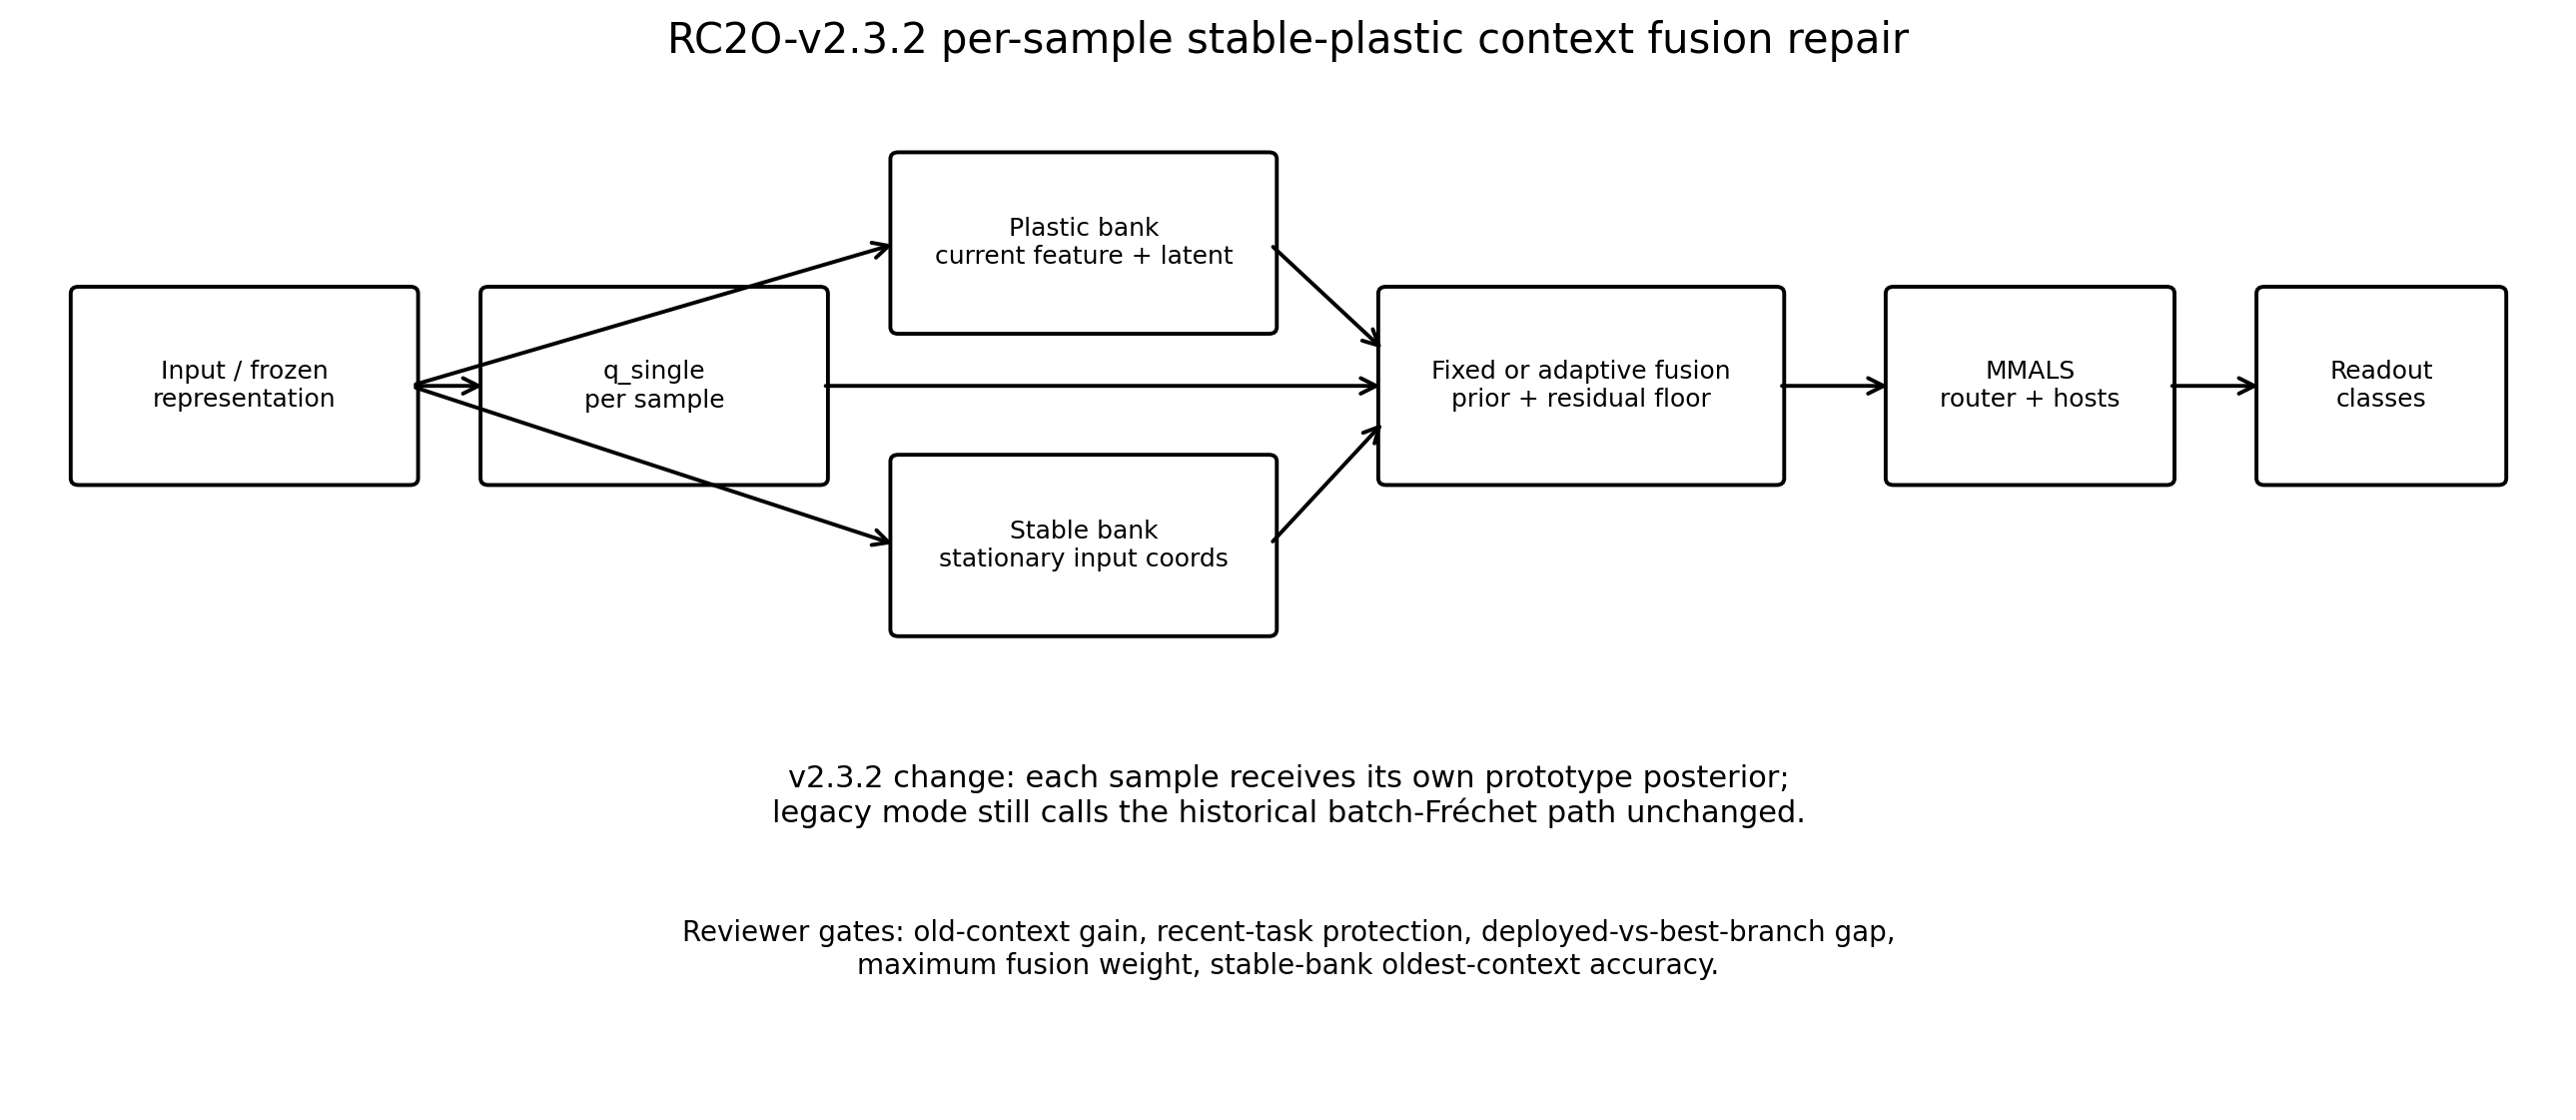
\includegraphics[width=\textwidth]{../figures/v232_architecture_flow.png}
\caption{The repaired context-memory path. New modes use per-sample evidence. Legacy mode retains the historical batch-Fr\'echet implementation.}
\end{figure}

The module consumes the representation entering MMALS and produces a deployed context posterior. Three evidence families are available:

\begin{enumerate}[leftmargin=1.5em]
\item \textbf{Single-input branch}: the existing learned context encoder, already per sample.
\item \textbf{Plastic branch}: per-sample evidence in current learned feature and mediated-latent coordinates.
\item \textbf{Stable branch}: per-sample evidence in a stationary input representation. For external visual datasets this is the frozen feature-backbone output; for the MNIST family it is the fixed input vector.
\end{enumerate}

\section{Per-sample prototype evidence}

For sample $x$ and diagonal context statistics $(\mu_c,\sigma_c^2)$, v2.3.2 uses the dimension-normalized energy

\begin{equation}
E_c(x)=\frac{1}{d}\sum_{j=1}^{d}
\left[
\frac{(x_j-\mu_{c,j})^2}{\max(\sigma^2_{c,j},\epsilon)}
+\log\max(\sigma^2_{c,j},\epsilon)
\right].
\end{equation}

The context posterior is

\begin{equation}
q_{\mathrm{proto}}(c\mid x)=
\frac{\exp(-E_c(x)/\tau)}{\sum_k \exp(-E_k(x)/\tau)}.
\end{equation}

This creates a matrix with shape \code{[batch, contexts]}; each sample can receive a different context assignment inside the same replay batch.

\lstinputlisting[caption={Dimension-normalized per-sample diagonal Gaussian energy.}]{snippets/_spcm_sample_diag_energy.py}

\lstinputlisting[caption={Per-sample posterior over all available context prototypes.}]{snippets/_spcm_sample_posterior.py}

\section{Stable and plastic memory semantics}

\subsection{Plastic bank}

The plastic bank is refreshed from the current model and represents the latest learned geometry. It can adapt quickly but may drift.

\subsection{Stationary stable bank}

The stationary stable bank stores statistics in the representation entering MMALS. It is deliberately outside the continually updated context encoder and mediated-latent geometry. The bank is frozen after first creation for each context in the principal stationary variants.

This does not guarantee that the stable bank will solve context retention. It creates a falsifiable test of whether a non-drifting coordinate system is more useful than frozen statistics in moving coordinates.

\section{Fusion controls}

\subsection{Fixed fusion}

The fixed-fusion row uses

\begin{equation}
q_{\mathrm{deploy}}=0.10q_{\mathrm{single}}+0.35q_{\mathrm{plastic}}+0.55q_{\mathrm{stable}}.
\end{equation}

This row tests the banks before asking whether a trainable gate adds value.

\subsection{Adaptive fusion with a residual prior floor}

The unconstrained gate produces $\tilde{w}=\operatorname{softmax}(g(m))$. v2.3.2 uses

\begin{equation}
w=\rho w_{\mathrm{prior}}+(1-\rho)\tilde{w},
\end{equation}

with $w_{\mathrm{prior}}=(0.10,0.35,0.55)$ and $\rho=0.35$. The final layer is initialized so that the unconstrained gate also starts at the prior. Under these values, no branch can exceed 0.8425, which is below the reviewer cap of 0.85.

\lstinputlisting[caption={Fusion implementation with exact legacy mode and residual-prior adaptive mode.},firstline=1,lastline=120]{snippets/StablePlasticContextMemory.py}

\section{Training-path repair}

The v2.3.1 main current-task loss used the inherited historical forward path even for non-legacy candidates. The new module received gradients mainly through auxiliary replay/context losses. In v2.3.2, legacy keeps the exact historical path, while non-legacy candidates train through the same deployed posterior used at evaluation.

\lstinputlisting[caption={Backward-compatible training dispatch.}]{snippets/deployed_training_dispatch.py}

This is still a localized change: the host networks, fungal transformations, router, global readout, task loss, replay structures and representation control remain inherited.

\section{Ablation matrix}

\begin{longtable}{p{4.1cm}p{2.6cm}p{3.1cm}p{4.2cm}}
\toprule
\textbf{Variant} & \textbf{Fusion} & \textbf{Stable coordinates} & \textbf{Purpose} \\
\midrule
\endfirsthead
\toprule
\textbf{Variant} & \textbf{Fusion} & \textbf{Stable coordinates} & \textbf{Purpose} \\
\midrule
\endhead
\code{legacy\_reference} & Historical & Historical learned coordinates & Exact reproduction reference. \\
\code{deployed\_posterior\_distill} & Historical & Historical & Preserve the strongest legacy-style context-distillation control. \\
\code{stable\_plastic\_fixed\_fusion} & Fixed 0.10/0.35/0.55 & Stationary input & Test repaired banks without a trainable gate. \\
\code{per\_sample\_adaptive\_fusion} & Prior-floor adaptive & Dynamic learned feature/latent & Isolate the effect of per-sample evidence and constrained gating. \\
\code{per\_sample\_adaptive\_stationary\_stable} & Prior-floor adaptive & Stationary input & Principal repaired candidate. \\
\code{oracle\_context\_diagnostic} & Oracle & Oracle & Non-deployable upper-bound diagnostic. \\
\bottomrule
\end{longtable}

The full profile additionally provides stable-only and plastic-only controls.

\section{Reviewer promotion gates}

All inherited v2.3.1 gates remain active:

\begin{itemize}[leftmargin=1.5em]
\item oldest-two context top-1 gain at least 0.20;
\item oldest-two task accuracy gain at least 0.03;
\item at least two fewer zero-recall classes;
\item average-accuracy regression no worse than 0.02;
\item recent-two regression no worse than 0.03;
\item confident-collapse reduction at least 0.10.
\end{itemize}

Three new gates are added:

\begin{itemize}[leftmargin=1.5em]
\item deployed context accuracy must be within 0.05 of the best component branch;
\item average maximum fusion weight must not exceed 0.85;
\item variants claiming a stationary stable bank must obtain oldest-two stable-bank context top-1 of at least 0.20.
\end{itemize}

These rules prevent a candidate from being promoted merely because another branch compensates for a non-functional stable bank or because the fused output discards stronger internal evidence.

\section{Optional compact PyTorch persistence}

The default remains

\begin{lstlisting}
V232_PT_SAVE_POLICY = "off"
\end{lstlisting}

The recommended audit setting is

\begin{lstlisting}
V232_PT_SAVE_POLICY = "final"
V232_PT_VARIANT_ALLOWLIST = [
    "legacy_reference",
    "per_sample_adaptive_stationary_stable",
]
V232_PT_INCLUDE_REPLAY_MEMORY = False
\end{lstlisting}

This produces one compact final checkpoint per selected variant and seed. The checkpoint is intended for a separate host-specialization audit and contains the model, context-memory module, banks, audit memory, configuration and run metadata. It omits optimizer state and full replay memory by default.

\section{Execution sequence}

\begin{enumerate}[leftmargin=1.5em]
\item Run the CORe50 mechanism matrix on seeds 0 and 4.
\item Compare fixed fusion against legacy to establish whether the repaired banks are useful without a learned gate.
\item Compare stationary adaptive fusion against fixed fusion to measure the incremental value of adaptive selection.
\item Promote only if every reviewer gate passes.
\item Run one-seed regression smokes on MNIST, FashionMNIST, RotatedMNIST and PermutedMNIST.
\item Protect the robust SplitCIFAR10 result with explicit non-regression criteria.
\item Use SplitCIFAR100 diagnostically, because representation and 100-class readout limitations remain unresolved.
\item Return to five-seed CORe50 only after the cross-dataset regression checks.
\end{enumerate}

\section{Tracked changes}

\begin{longtable}{p{1.6cm}p{2.8cm}p{5.2cm}p{5.2cm}}
\toprule
\textbf{ID} & \textbf{Area} & \textbf{v2.3.1} & \textbf{v2.3.2} \\
\midrule
\endfirsthead
\toprule
\textbf{ID} & \textbf{Area} & \textbf{v2.3.1} & \textbf{v2.3.2} \\
\midrule
\endhead
V232-001 & Prototype evidence & One batch-level posterior copied over the batch. & Per-sample diagonal-Gaussian evidence in repaired modes. \\
V232-002 & Stable coordinates & Stable values in drifting learned coordinates. & Optional frozen input-representation stable bank. \\
V232-003 & Adaptive fusion & Unconstrained gate could suppress branches. & Prior initialization and residual prior floor. \\
V232-004 & Training path & Main task loss used inherited legacy forward path. & Non-legacy task loss uses deployed posterior. \\
V232-005 & Reviewer gates & No branch-gap or gate-collapse criterion. & Branch-gap, fusion-weight and stable-old-context gates. \\
V232-006 & Persistence & Optional compact final checkpoints. & Same policy with v2.3.2 versioned metadata and manifest. \\
\bottomrule
\end{longtable}

\section{Reproducibility and static validation}

The generated notebook has 96 cells, including 44 executable cells. The notebook JSON was parsed successfully and every code cell passed Python syntax validation after notebook shell and magic lines were excluded from compilation. Outputs and execution counts from the predecessor were cleared to prevent stale evidence from appearing as v2.3.2 results.

The notebook also includes runtime self-tests for:

\begin{itemize}[leftmargin=1.5em]
\item exact legacy fusion equivalence;
\item per-sample prototype assignments that differ within one batch;
\item normalized posteriors across arbitrary context counts;
\item the adaptive fusion-weight cap implied by the residual prior floor;
\item absence of dataset-specific fields in the context-memory configuration;
\item normalized overlap-aware targets.
\end{itemize}

\section{Archive contents}

The accompanying GitHub package contains:

\begin{itemize}[leftmargin=1.5em]
\item the new notebook;
\item this compiled PDF and LaTeX source;
\item architecture and evidence figures;
\item compact v2.3.1 CSV evidence used in the report;
\item repository README, changelog and implementation notes;
\item a SHA-256 file manifest.
\end{itemize}

\section{Final scientific position}

RC2O-v2.3.1 should be retained as a positive but failed-gate result. It demonstrated that stable-plastic training can improve retention and class coverage, but it did not validate the intended adaptive fusion mechanism. RC2O-v2.3.2 therefore does not discard the stable-plastic hypothesis. It isolates and repairs the evidence granularity, coordinate stability and training-path issues that prevented a fair test.

The correct next claim is narrow and falsifiable:

\begin{quote}
Per-sample prototype evidence and a stationary stable context bank may allow MMALS to preserve the old-context gains observed in v2.3.1 while avoiding prototype-branch suppression and excessive recent-task regression.
\end{quote}

Whether that statement is supported depends entirely on the future execution and the predefined gates.

\end{document}
